\documentclass{article}
\usepackage{graphicx} % Required for inserting images
\usepackage[utf8]{inputenc}
\usepackage{hyperref}


\title{Bookig App}
\author{Andrea Gepponi}
\date{Maggio - Giugno 2024}

\usepackage{geometry}
 \geometry{
 a4paper,
 total={170mm,257mm},
 left=20mm,
 top=20mm,
 }

\begin{document}

\maketitle

\begin{figure}[h!]
    \centering
    \includegraphics[width=0.5\textwidth]{unifi-logo.png}
\end{figure}

\newpage

\renewcommand{\contentsname}{Index}
\tableofcontents

\newpage

\section{Introduzione}
Elaborato per il superamento dell’esame di Ingegneria del Software, appartenente al modulo Basi di Dati / Ingegneria del Software del corso di Laurea Triennale in Ingegneria Informatica dell’Università degli Studi di Firenze.
\vspace{4mm}
Il progetto è stato sviluppato da Andrea Gepponi, matricola 7047622, durante il periode Maggio - Giugno 2024 (a.a. 2023/2024).
\vspace{4mm}
\newline
Il codice sorgente è disponibile al seguente link:

\vspace{4mm}
\subsection{Obbiettivo e descrizione progetto}
Il progetto consiste in un programma che permette di mettere a disposizione delle strutture alberghiere e prenotare  stanze.
\vspace{0mm}
\newline
Comprende un sistema a più utenti che possono aggiungere strutture effettuare prenotazioni e gestire il proprio profilo.
\vspace{0mm}
\newline
Gli utenti si suddividono in Manager e Customer.
\vspace{0mm}
\newline
Il Manager aggiunge strutture disponibili mentre il Customer effettua prenotazioni e lascia recenzioni.
\vspace{0mm}
\newline
Per la gestione e il salvataggio dei dati è stato creato e connesso un database.
\vspace{4mm}
\subsection{Struttura e pratiche utilizzate}
Il software `e stato sviluppato in Java, mentre per la gestione e il salvataggio dei dati `e stato
connesso un database PostgreSQL ed `e stata utilizzata la libreria JDBC (Java DataBase
Connectivity).
\vspace{2mm}
\newline
Per mantenere una separazione delle responsabilit`a, la struttura del progetto `e stata divisa
in tre parti principali: Business Logic, Domain Model e ORM. Questi tre packages si occupano in modo distinto della logica di business, della rappresentazione dei dati e dell’accesso
ai dati (Figura 1):
\begin{itemize}
    \item \textbf{Business Logic}: contiene le classi che implementano la logica di business del sistema.
    \item \textbf{Domain Model}: contiene le classi che rappresentano le entità del sistema.
    \item \textbf{ORM}: contiene le classi che implementano l’Object-Relational Mapping. In questo modo è possibile rendere i dati persistenti e recuperarli dal database.
\end{itemize}
\vspace{2mm}
Per utilizzare il software `e stata creata un’interfaccia da riga di comando (CLI) che permette di interagire con il sistema in modo semplice e intuitivo.
\vspace{0mm}
\newline
Gli Use Case Diagram e i Class Diagram seguono lo standard UML (Unified Modeling
Language) e sono stati realizzati con il software StarUML. Infine, per la parte di testing `e
stato utilizzato JUnit.
Le piattaforme e i software utilizzati sono stati:

\begin{itemize}
    \item IntelliJ IDEA: IDE per lo sviluppo in Java
    \item StarUML: software per la creazione di diagrammi UML
    \item Draw.io: altro software per la creazione di diagrammi
    \item PgAdmin: software per la gestione di database PostgreSQL
    \item GitHub: piattaforma per la condivisione del codice sorgente
    \item Lunacy: software per la creazione di mock-up
    \item tree.nathanfriend.io: sito per la creazione di diagrammi di directory
\end{itemize}
\begin{figure}[h!]
    \centering
    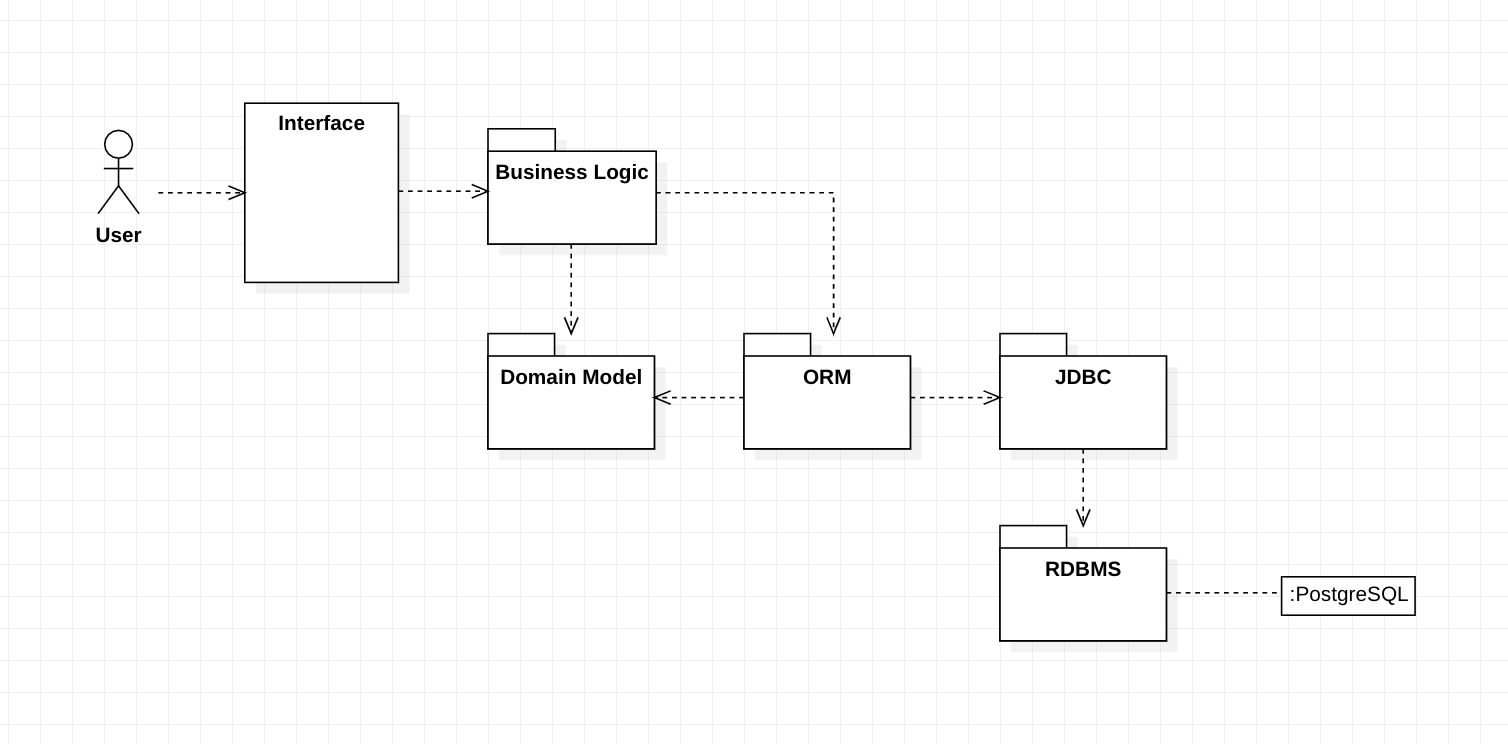
\includegraphics[width=1.0\textwidth]{package_dependency_diagram.png}
    \caption{Package Dependency Diagram}
    \label{fig:package_diagram}
\end{figure}
\newpage
\section{Progettazione}
\subsection{Use case Diagram}
Il funzionamento del sistema è mostrato nello use case diagram, sia lato Customer che lato Manager.
\begin{figure}[h!]
    \centering
    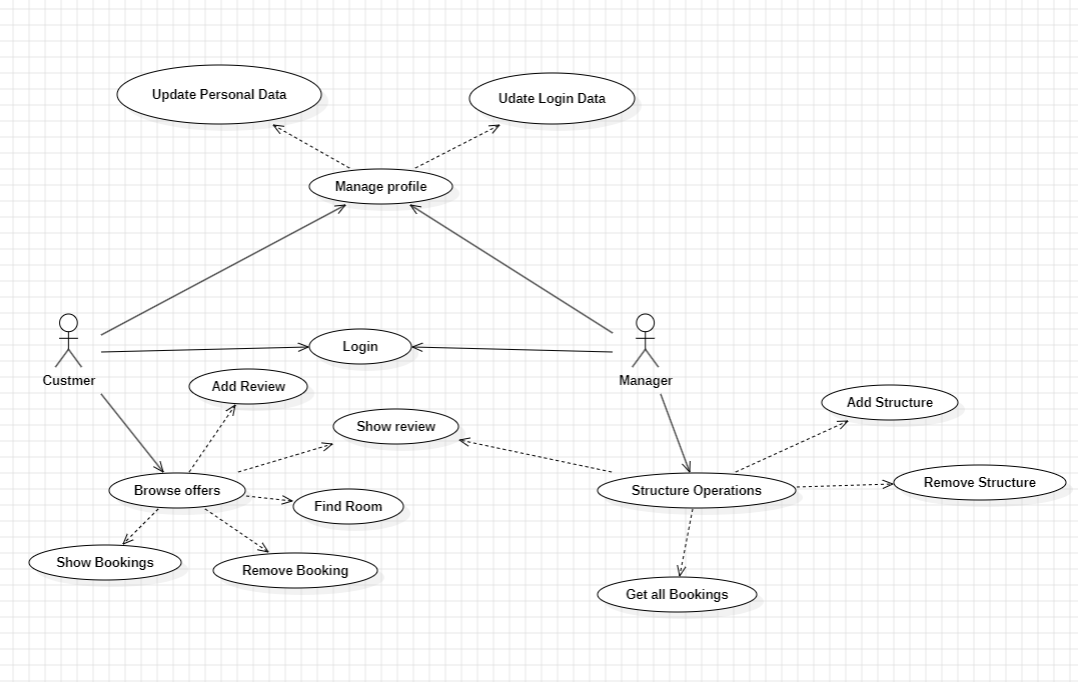
\includegraphics[width=1.0\textwidth]{UseCase.png}
    \caption{Use Case Diagram}
    \label{fig:use_case_diagram}
\end{figure}
\newpage
\subsection{Use Case Template}
Di seguito sono riportati i template di alcuni dei casi d’uso implementati, in ognuno possiamo trovare: una breve descrizione, il livello del caso d’uso, gli attori coinvolti, le precondizioni, le post-condizioni, il flusso base e, eventualmente, i flussi alternativi.
\begin{table}[h!]
    \centering
    \begin{tabular}{|l|p{10cm}|}
        \hline
        \textbf{Use Case \#1} & Accesso al sistema (Sign in) \\ \hline
        \textbf{Brief Description} & L’utente accede al sistema tramite le proprie credenziali\\ \hline
        \textbf{Level} & User Goal \\ \hline
        \textbf{Actors} & Customer, Manager \\ \hline
        \textbf{Pre-conditions} & L’utente deve essere nella pagina iniziale di accesso. \\ \hline
        \textbf{Basic Flow} & 
        \begin{enumerate}
            \item L’utente inserisce le proprie credenziali (username e password)
            \item L’utente preme il pulsante di accesso
            \item Il sistema verifica le credenziali
            \item Il sistema autentica l’utente
        \end{enumerate} \\ \hline
        \textbf{Alternative Flows} & 
        \begin{itemize}
            \item 3a. Se le credenziali fornite non sono corrette, il sistema mostra un messaggio di errore all’utente
        \end{itemize} \\ \hline
        \textbf{Post-conditions} & L’utente è autenticato nel sistema e ha accesso alle funzionalità riservate \\ \hline
    \end{tabular}
    \caption{Use Case Template 1 (Sign in)}
    \label{tab:use_case_1}
\end{table}
\begin{table}[h!]
    \centering
    \begin{tabular}{|l|p{10cm}|}
        \hline
        \textbf{Use Case \#2} & Registrazione nel sistema (Sign up) \\ \hline
        \textbf{Brief Description} & L’utente si registra nel sistema creando un nuovo account\\ \hline
        \textbf{Level} & User Goal \\ \hline
        \textbf{Actors} & Customer, Manager \\ \hline
        \textbf{Pre-conditions} & L’utente deve essere nella pagina iniziale di registrazione. \\ \hline
        \textbf{Basic Flow} & 
        \begin{enumerate}
            \item L’utente fornisce i dettagli richiesti per la registrazione
            \item L’utente conferma la registrazione
            \item Il sistema verifica i dati forniti
            \item Il sistema crea un nuovo account per l’utente
        \end{enumerate} \\ \hline
        \textbf{Alternative Flows} & 
        \begin{itemize}
            \item 3a. Se l’utente fornisce dati non validi o se l’email o lo username sono già utilizzati da un altro account, il sistema mostra un messaggiodi errore
        \end{itemize} \\ \hline
        \textbf{Post-conditions} &L’utente `e registrato nel sistema e pu`o accedere utilizzando le credenziali create durante la registrazione \\ \hline
    \end{tabular}
    \caption{Use Case Template 2 (Sign up)}
    \label{tab:use_case_2}
\end{table}
\newpage
\begin{table}[h!]
    \centering
    \begin{tabular}{|l|p{10cm}|}
        \hline
        \textbf{Use Case \#3} & Ricerca e prenotazione  di una stanza \\ \hline
        \textbf{Brief Description} & L’utente ricerca una stanza da prenotare e ne sceglie una.\\ \hline
        \textbf{Level} & Function \\ \hline
        \textbf{Actors} & Customer\\ \hline
        \textbf{Pre-conditions} & L’utente deve essere nella pagina di Browsing. \\ \hline
        \textbf{Basic Flow} & 
        \begin{enumerate}
            \item L’utente fornisce i dettagli della struttura
            \item Il sistema fornisce una lista di stanze che soddisfano le condizioni dell'utente
            \item L'utente decide se confermare la prenotazione o meno
        \end{enumerate} \\ \hline
        \textbf{Alternative Flows} & 
        \begin{itemize}
            \item 2a. Se non ci sono stanze disponibili viene generato un messaggio d'errore
        \end{itemize} \\ \hline
        \textbf{Post-conditions} &L'utente ha a prenotato una stanza\\ \hline
    \end{tabular}
    \caption{Use Case Template 3 (Browsing)}
    \label{tab:use_case_3}
\end{table}
\begin{table}[h!]
    \centering
    \begin{tabular}{|l|p{10cm}|}
        \hline
        \textbf{Use Case \#4} & Cancellazione di una prenotazione \\ \hline
        \textbf{Brief Description} & L’utente cancella una sua prenotazione.\\ \hline
        \textbf{Level} & User goal \\ \hline
        \textbf{Actors} & Customer\\ \hline
        \textbf{Pre-conditions} & L’utente deve essere nella pagina di Browsing. \\ \hline
        \textbf{Basic Flow} & 
        \begin{enumerate}
            \item L’utente fornisce il nome della struttura e il periodo della prenotazione.
        \end{enumerate} \\ \hline
        \textbf{Post-conditions} &L'utente ha rimosso una prenotazione.\\ \hline
    \end{tabular}
    \caption{Use Case Template 4 (Deleting)}
    \label{tab:use_case_4}
\end{table}
\begin{table}[h!]
    \centering
    \begin{tabular}{|l|p{10cm}|}
        \hline
        \textbf{Use Case \#5} & Aggiunta di una struttura \\ \hline
        \textbf{Brief Description} & L’utente aggiunge una struttura al database.\\ \hline
        \textbf{Level} & User goal \\ \hline
        \textbf{Actors} & Manager\\ \hline
        \textbf{Pre-conditions} & L’utente deve essere nella pagina di Action. \\ \hline
        \textbf{Basic Flow} & 
        \begin{enumerate}
            \item L’utente fornisce i dati della struttura da inserire.
        \end{enumerate} \\ \hline
        \textbf{Post-conditions} &L'utente ha aggiunto una struttura.\\ \hline
    \end{tabular}
    \caption{Use Case Template 5 (Adding Structure)}
    \label{tab:use_case_5}
\end{table}
\newpage
\subsection{Mockups}
Ecco di seguito alcuni possibili Mock-ups relativi alle interfacce grafiche del sistema.
\begin{figure}[h!]
    \centering
    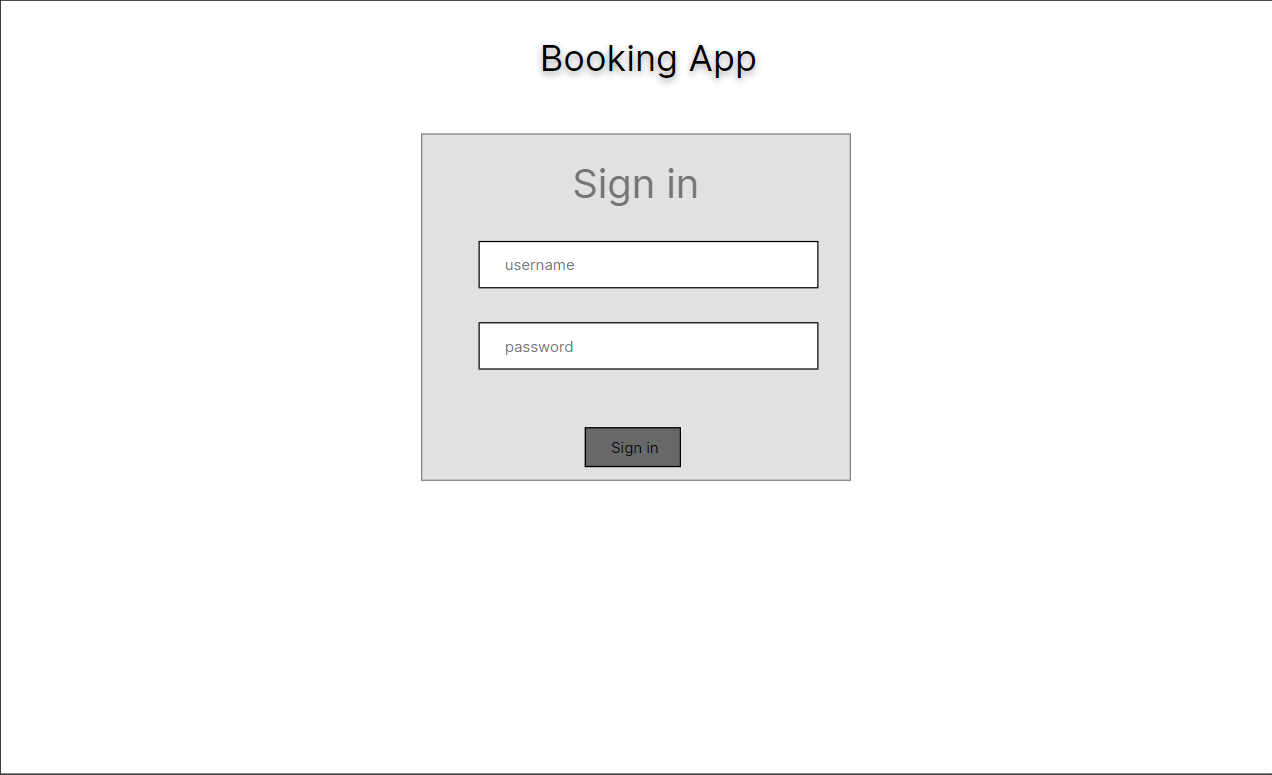
\includegraphics[width=0.8\textwidth]{SignIn.png}
    \caption{Sign in mockup}
    \label{fig:Sign in mockup}
\end{figure}
\begin{figure}[h!]
    \centering
    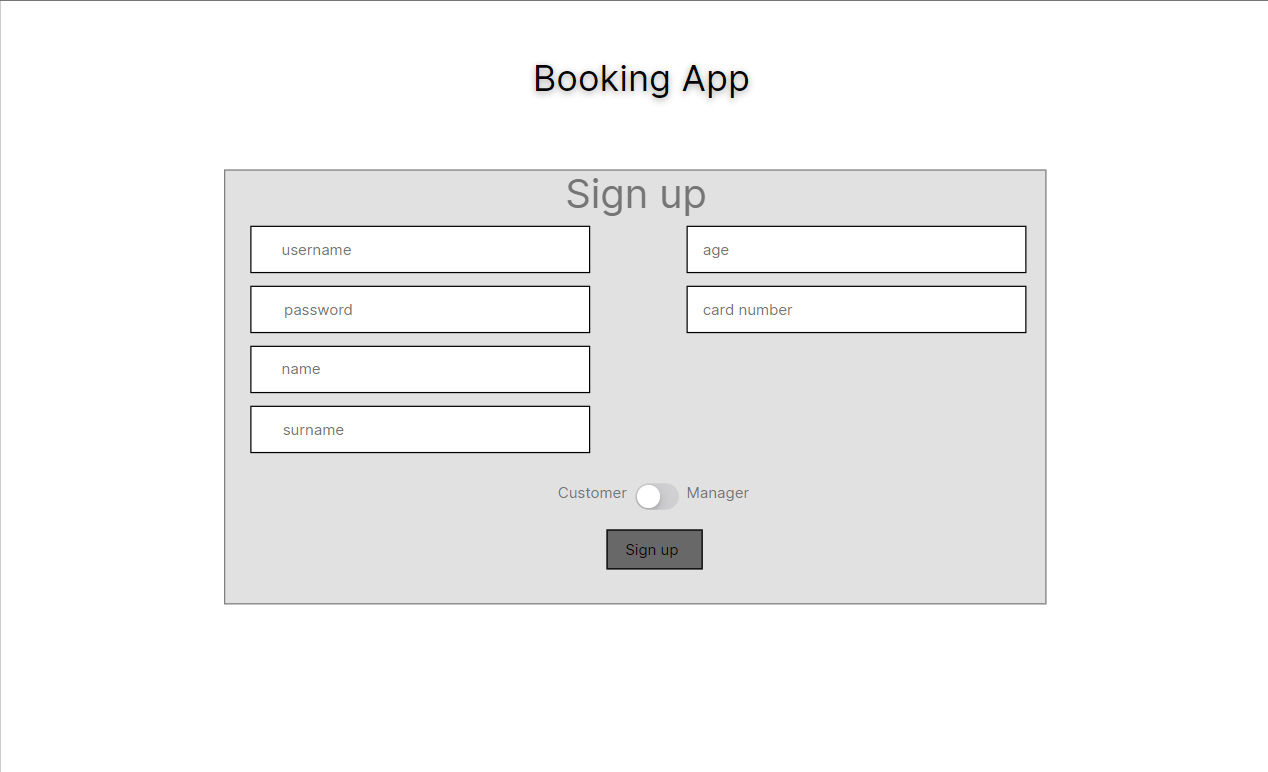
\includegraphics[width=0.8\textwidth]{SignUp.png}
    \caption{Sign up mockup}
    \label{fig:Sign up mockup}
\end{figure}
\newpage
\begin{figure}[h!]
    \centering
    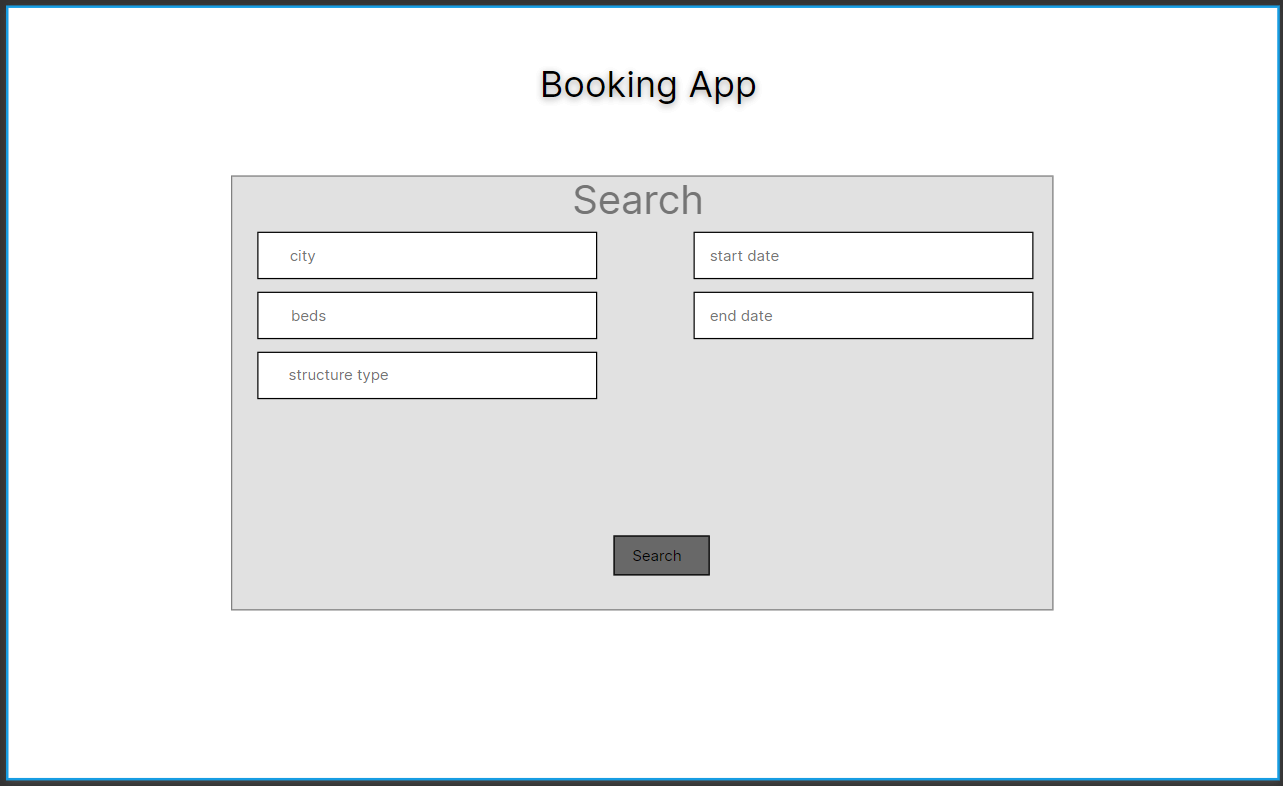
\includegraphics[width=0.8\textwidth]{Search.png}
    \caption{Search mockup}
    \label{fig:Search mockup}
\end{figure}
\vspace{40mm}
\begin{figure}[h!]
    \centering
    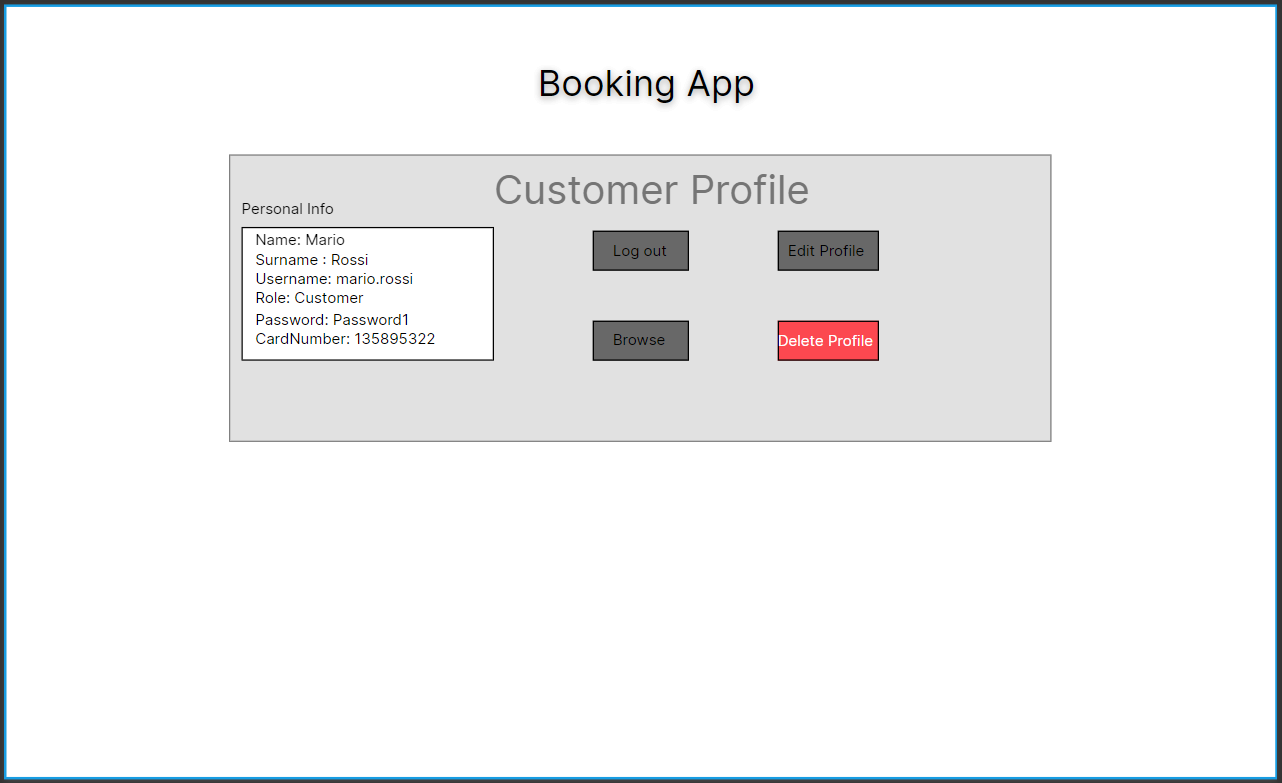
\includegraphics[width=0.8\textwidth]{CustomerProfile.png}
    \caption{Profile mockup}
    \label{fig:Profile mockup}
\end{figure}
\newpage
\subsection{Class Diagram}
Il softwere si suddivide in tre packages, di seguito il diagramma delle classi di ciascuno di essi:
\begin{itemize}
    \item Business Logic:contiene le classi che implementano la logica di business del sistema, ovvero i seguenti controller:quello che gestisce l’accesso e la registrazione dei nuovi utenti (LoginController),quello che permette ai Customer di cercare e prenotare stanze, di aggiungere e leggere recenzioni(CustomerProfileController),quello che permette ai Manager di aggiungere e rimuovere strutture e leggere recenzioni (ManagerProfileController).
    \item Domain Model:contiene le classi che rappresentano le entità del sistema, ovvero:Customer, Manager, CreditCard, Review, Period, Booking,Room, Structure.Contiene anche BookingMapper che implementa il mapper per le prenotazioni.
    \item ORM:contiene le classi che implementano l’Object-Relational Mapping, quindi contiene una classe per ogni entit`a del sistema:CustomerDAO, ManagerDAO,CreditCardDAO,ReviewDAO, StructureDAO, RoomDAO, BookingDAO. Contiene anche la classe ConnectionManager che si occupa di gestire la connessione al database.
\end{itemize}

\begin{figure}[h!]
    \centering
    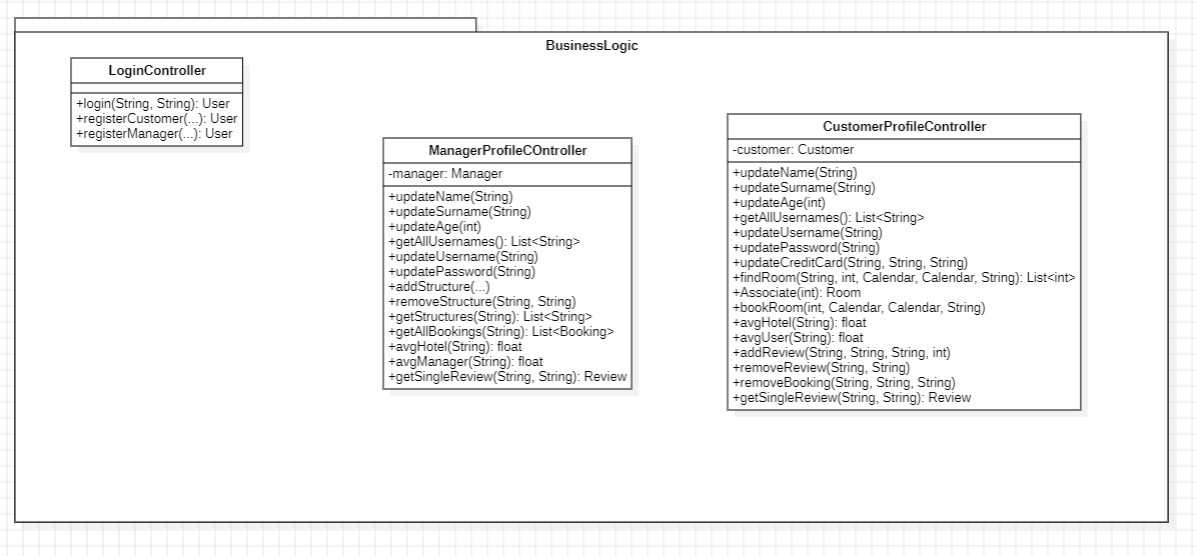
\includegraphics[width=1.0\textwidth]{BusinessLogic.png}
    \caption{Business Logic Diagram}
    \label{fig:BusinessLogic}
\end{figure}
\begin{figure}[h!]
    \centering
    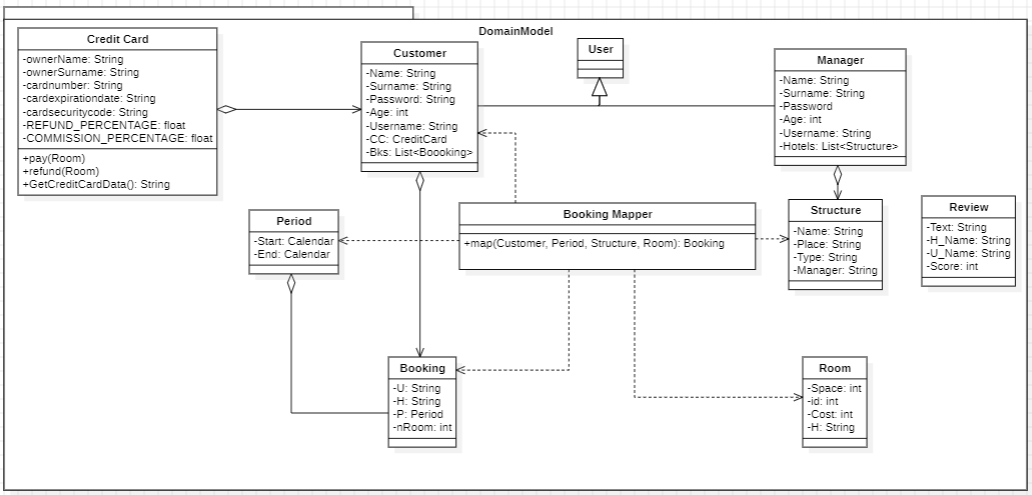
\includegraphics[width=1.0\textwidth]{Domain_Model.png}
    \caption{Domain Model Diagram}
    \label{fig:DomainModel}
\end{figure}
\begin{figure}[h!]
    \centering
    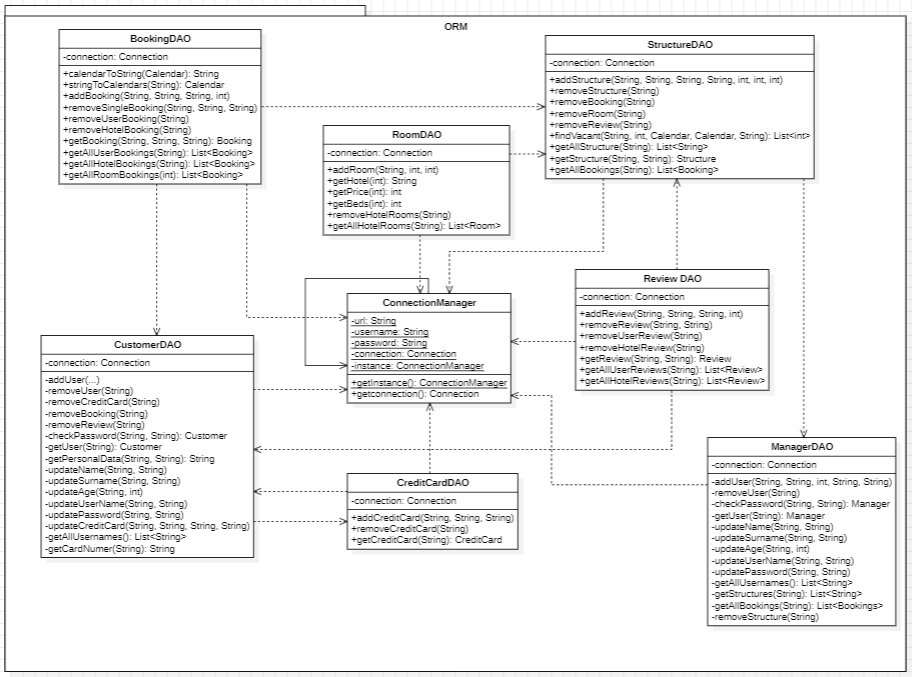
\includegraphics[width=1.0\textwidth]{ORM.png}
    \caption{ORM Diagram}
    \label{fig:ORM}
\end{figure}
\newpage

\subsection{ER Diagram}
Per la progettazione del database è stato realizzato un ER diagram.
\begin{itemize}
    \item User:rappresenta sia l'entità Customer che Manager, distinte dall'attributo "role".
    \item CreditCard: rappresenta l'entità CreditCard.
    \item Structure: rappresenta l'entità Structure.
    \item Room: rappresenta l'entità Room.
    \item Booking: risolve la relazione Booking tra Structure, Booking e Room.
    \item Review: risolve la relazione Review tra User e Structure.
\end{itemize}
\begin{figure}[h!]
    \centering
    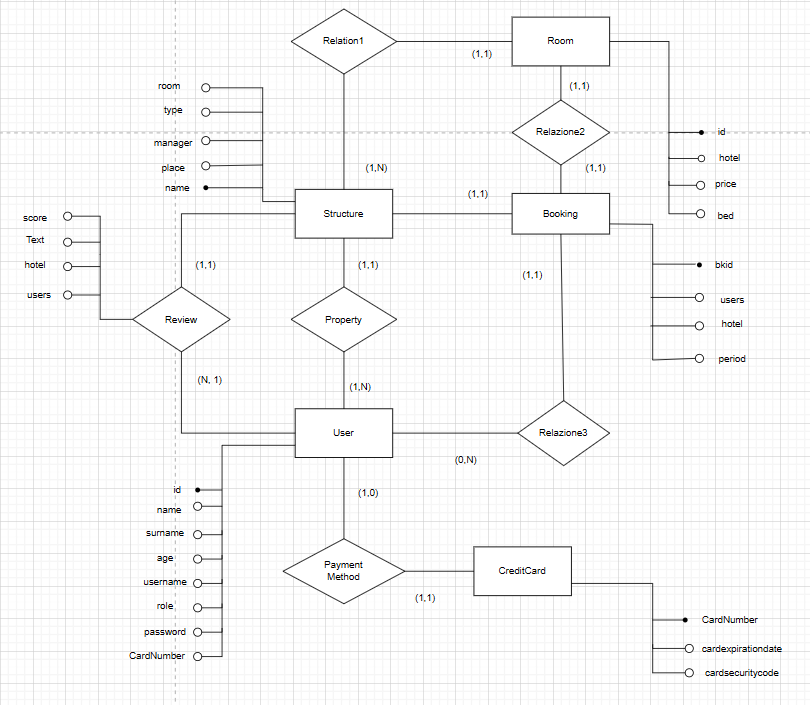
\includegraphics[width=1.0\textwidth]{ER-2.png}
    \caption{ER Diagram}
    \label{fig:ER-Diagram}
\end{figure}
\newpage
\subsection{Navigation Diagram}
Il seguente diagramma rappresenta quelle che sono le pagine principali del sistema e le possibili azioni che l'utente può compiere. Sono anche rappresentati i modi con cui si pu`o navigare tra le varie pagine.\newline
Alcune pagine sono:
\begin{itemize}
    \item la pagina iniziale: dove l’utente pu`o registrarsi o effettuare il login.
    \item User Page: da dove si può accedere al profilo o alle azioni.
    \item Profile Editor: da dove possono essere modificate le informazioni del profilo.
\end{itemize}
\begin{figure}[h!]
    \centering
    \includegraphics[width=1.0\textwidth]{Navigation.png}
    \caption{Navigation Diagram}
    \label{fig:Navigation Diagram}
\end{figure}
\newpage
\subsection{Struttura della directory}
Di seguito la struttura della directory che contiene:
\begin{itemize}
    \item src: contiene il codice sorgente.
    \item test: contiene il codice di test.
\end{itemize}
\begin{figure}[h!]
    \centering
    \includegraphics[width=0.4\textwidth]{filemap.png}
    \caption{directory structure}
    \label{fig:directory structure}
\end{figure}
\newpage
\section{Implementazione}
\subsection{Domain Model}
Nel package Domain Model sono state implementate le classi che rappresentano le entit`a del sistema.
\subsubsection{User}
La classe User è una classe astratta che permette di semplificare l'operazione di login degli utenti.
\subsubsection{Customer}
La classe Customer rapprresenta un utente che si è registrato nel sistema con l'intento di effettuare prenotazioni. I campi sono name, surname, Password, Age, Username, CC(CreditCard), e Bks(lista di prenotazioni).
\subsubsection{Manager}
La classe Manager rappresenta un utente che si è registrato nel sistema con l'intento di mettere disposizione strutture per le prenotazioni. I campi sono Name, Surname, Password, Age, Username e Hotels(lista di strutture).
\subsubsection{CreditCard}
La classe CreditCard rappresenta una carta di credito associata ad un Customer, utilizzata per i pagamenti.
\subsubsection{Structure}
La classe Structure rappresenta una struttura messa a disposizione da un Manager. I campi sono Name, Place, Type e Manager.
\subsubsection{Room}
La classe Room rappresenta una stanza di una struttura che è possibile prenotare. I campi sono Space(numero di posti letto), id, Cost e H(nome della struttura a cui appartengono).
\subsubsection{Review}
La classe Review rappresenta una recenzione lasciata da un utente ad una struttura. I campi sono Text, HName, UName e Score.
\subsubsection{Period}
La classe Period rappresenta l'intervallo di tempo per il quale un Customer intende prenotare una stanza. I campi sono Start e End.
\subsubsection{Booking e BookingMapper}
Booking rappresenta una prenotazione effettuata da un Customer su una determinata stanza di una struttura per un determinato periodo. I campi sono U(username del Customer), H(nome della struttura), P(periodo) e nRoom(id della stanza prenoata). La classe BookingMapper è stata creata per mappare i dati della prenotazione.
\begin{figure}[h!]
    \centering
    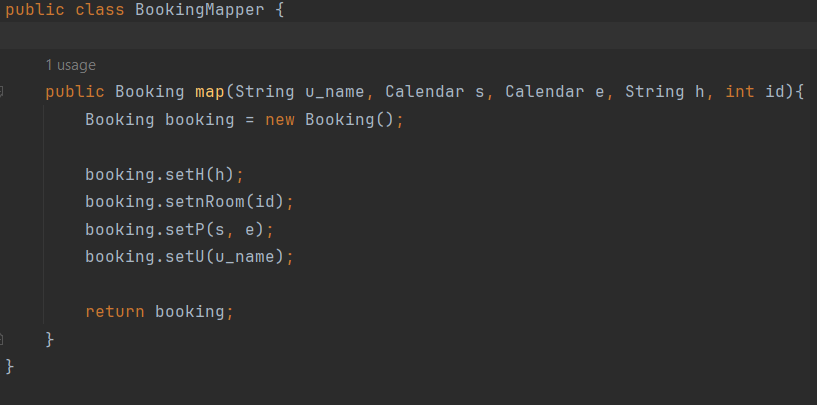
\includegraphics[width=1.0\textwidth]{mapper.png}
    \caption{Snippet di BookingMapper}
    \label{fig:mapper}
\end{figure}
\subsection{BusinessLogic}
Nel package BusinessLogic sono state implementate le classi che gestiscono la logica di business del sistema.
\subsubsection{LoginController}
Questa classe controlla la gestione dell'accesso e della registrazione degli utenti tramite le funzioni login(), registerCustomer() e registerManager(): la prima riceve in ingresso l'username, la password e il ruolo (Customer / Manager) dell'utente e controlla la correttezza delle cradenziali nel database, le altre due ricevono in ingresso tutti i dati dell'utente e li inseriscono nel database.
\subsubsection{CustomerProfileController}
Questa classe si occupa di tutte le azioni che possono essere effettuate da un Customer, permette di aggiornare i dati personali tramite le funzioni updateName(), updateSurname(), updateAge(), updateUsername(), updatePassword(), updateCreditCard(). Permette di ricercare stanze disponibili con la funzione findRoom() che richiede la città, la data di inizio e fine di prenotazione, il tipo di struttura e il numero di posti letto. Permette di prenotare una stanza tramite le funzioni associate()(che associa ad ogni id la stanza corrispondente) e bookRoom() che aggiunge una prenotazione. Permette infine di aggiungere e rimuovere recenzioni tramite addReview() e removeReview(), di cercare una singola recenzione tramite getSinglereview() e di vedere il punteggio medio di una determinata struttura e il punteggio medio delle recenzioni lasciate da un singolo utente tramite avgHotel() e avgUser().
\subsubsection{ManagerProfileController}
Questa classe gestisce tutte le azioni che possono essere effettuate da un Manager,permette di aggiornare i dati personali tramite le funzioni updateName(), updateSurname(), updateAge(), updateUsername(), updatePassword(). Permette di aggiungere e rimuovere strutture tramite addStructure e removeStructure. Permette di cercare singole recenzioni e di vedere il punteggio medio di una struttura tramite getSinglereview() e avgHotel. Permette infine di visualizzare tutte le prenotazioni per per una struttura tramite getAllBookings.
\subsection{Object-Relational Mapping}
Nel package ORM sono state implementate le classi che si occupano dell'Object-Relational Mapping, cioè delle operazioni di lettura e scrittura dati nel database.
\subsubsection{ConnectionManager}
La classe si occupa di gestire la connessione al database per le altre classi DAO tramite
il metodo getConnection(). Contiene inoltre i dati di accesso al database, ovvero URL,
username e password, che vengono utilizzati per stabilire la connessione. Per garantire
che ci sia una sola istanza della classe in tutto il sistema e quindi per evitare conflitti tra
connessioni, la classe `e implementata come un singleton.
\begin{figure}[h!]
    \centering
    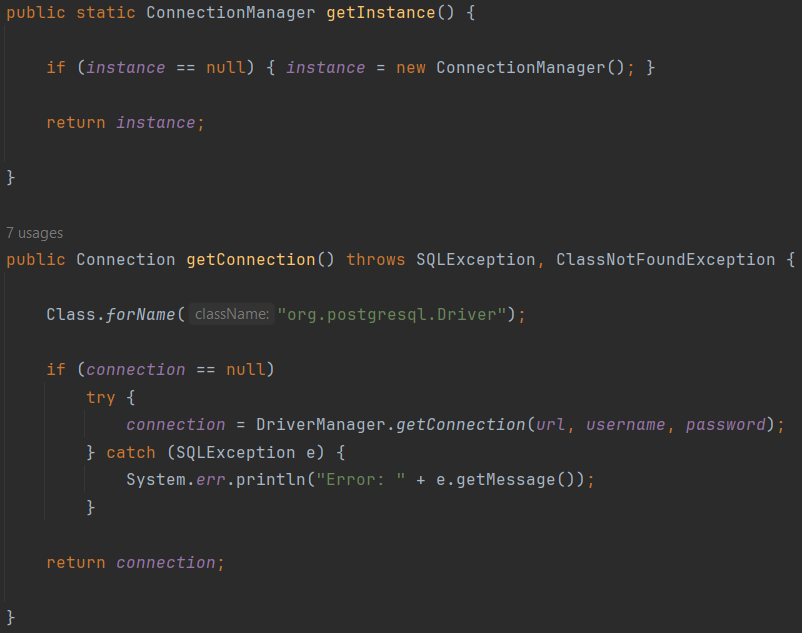
\includegraphics[width=0.7\textwidth]{ConnectionManager.png}
    \caption{Snippet di ConnectionManager}
    \label{fig:ConnectionManager}
\end{figure}
\subsubsection{CustomerDAO e ManagerDAO}
Queste due classi si occupano della gestione dei dati degli utenti, come le altre classi DAO permettono alle classi del package BusinessLogic di accedere ai dati salvati nel database. Entrambe le classi contengono metodi per l'aggiornamento di dati personali e per aggiungere o rimuovere utenti. In alcuni metodi vengono utilizzati anche altri DAO, per esempio quando viene rimosso un Customer viene rimossa anche la carta di credito associata insieme alle recenzioni e prenotazioni fatte da quel Customer.
\begin{figure}[h!]
    \centering
    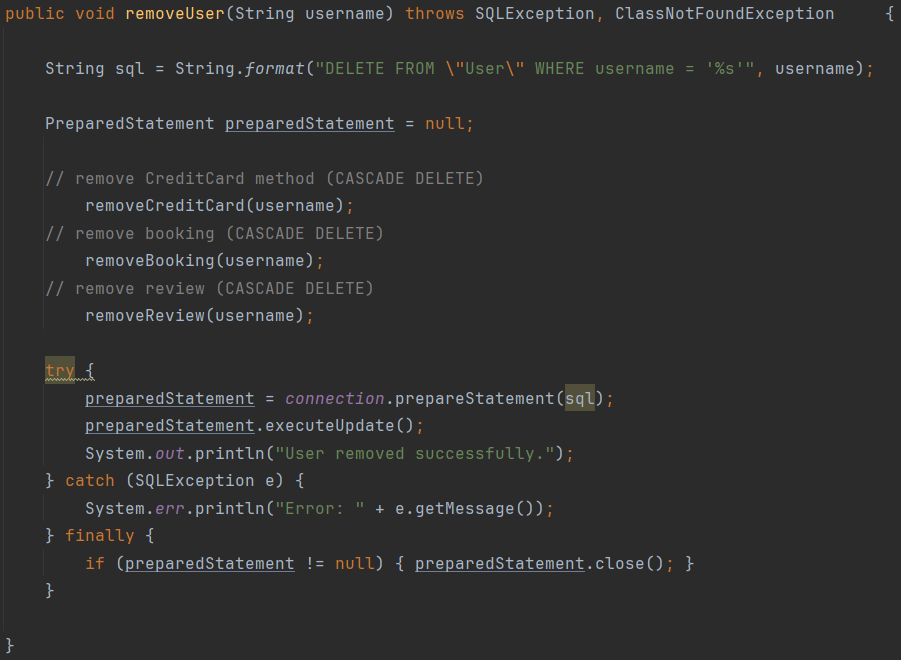
\includegraphics[width=0.7\textwidth]{CustomerDAO.png}
    \caption{Snippet di CustomerDAO}
    \label{fig:CustomerDAO}
\end{figure}
\subsubsection{BookingDAO}
La classe BookingDAO si occupa della gesione dei dati delle prenotazioni e permette alle classi della BusinessLogic di accedere ai dati delle prenotazioni salvati neldatabase. Contiene metodi come addBooking(), removeBooking(), getSingleBooking(), e metodi come calendarToString per convertire oggetti java.Calendar in stringhe da salvare nel database.
\subsubsection{CreditCardDAO}
Questa classe si occupa della gestione della carta di credito associata ad un Customer. Contiene i metodi addCreditCard(), removeCreditCard() e getCreditCard().
\subsubsection{StructureDAO}
La classe StructureDAO gestisce i dati relativi alle strutture e contiene metodi che permettono di cercare stanze libere findVacant() e ottenere tutte le prenotazioni su stanze di quella struttura getAllBooking(). Anche in questo caso vengono utilizzati altri DAO, quando una struttura viene rimossa vengono rimosse tutte le stanze, prenotazioni e recenzioni associate ad essa.
\begin{figure}[h!]
    \centering
    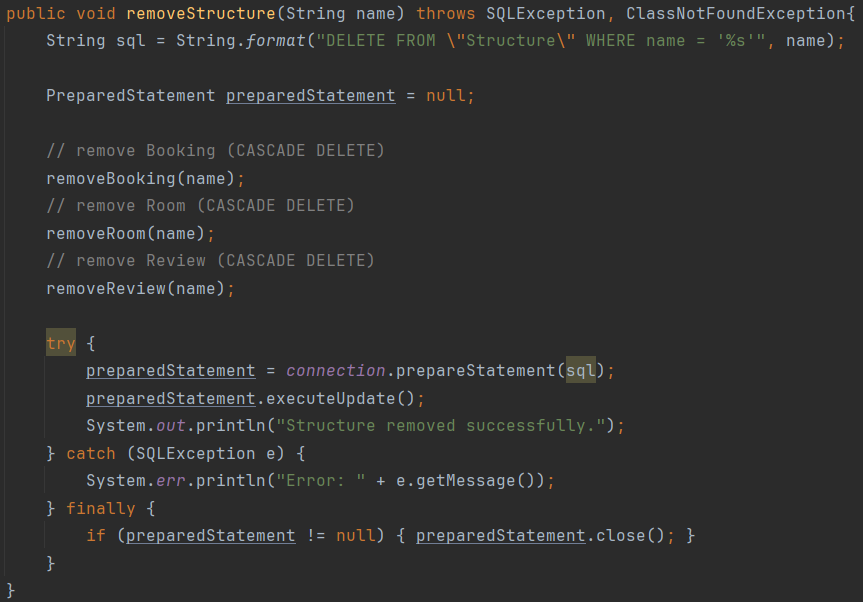
\includegraphics[width=0.7\textwidth]{StructureDAO.png}
    \caption{Snippet di StructureDAO}
    \label{fig:StructureDAO}
\end{figure}
\subsubsection{RoomDAO}
La classe RoomDAO si occupa dei dati relativi alle stanze. Contiene metodi come getPrice(), getHotel(), getBeds().
\subsubsection{ReviewDAO}
La classe ReviewDAO permette di ottenere una singola recenzione oppure ottenere recenzioni di un determinato Utente o di una determinata struttura tramite i metodi getReview(), getAllUserReview, getAllHotelReview(). Altri metodi permettono l'aggiunta di una recenzione o la rimozione di una o più recenzioni.
\subsection{Interfaccia CLI}
Per l'utilizzo del sistema è stata implementata un'interfaccia a linea di comando nel file main.java. L’utente pu`o navigare tra le varie pagine e compiere le funzionalità del programma inserendo i vari comandi indicati dal sistema. Nella pagina iniziale si ha scelta tra effettuare il login come Customer o come Manager, registrarsi come Customer o come Manager oppure chiudere il sistema. Ogni pagina è implementata tramite un ciclo do-while e uno switch-case per gestire le varie scelte dell'urente, mentre le varie funzionalità sono implementate con metodi specifici delle classi del package BusinessLogic. La
navigazione tra le pagine avviene tramite chiamate agli stessi metodi della classe main.
\begin{figure}[h!]
    \centering
    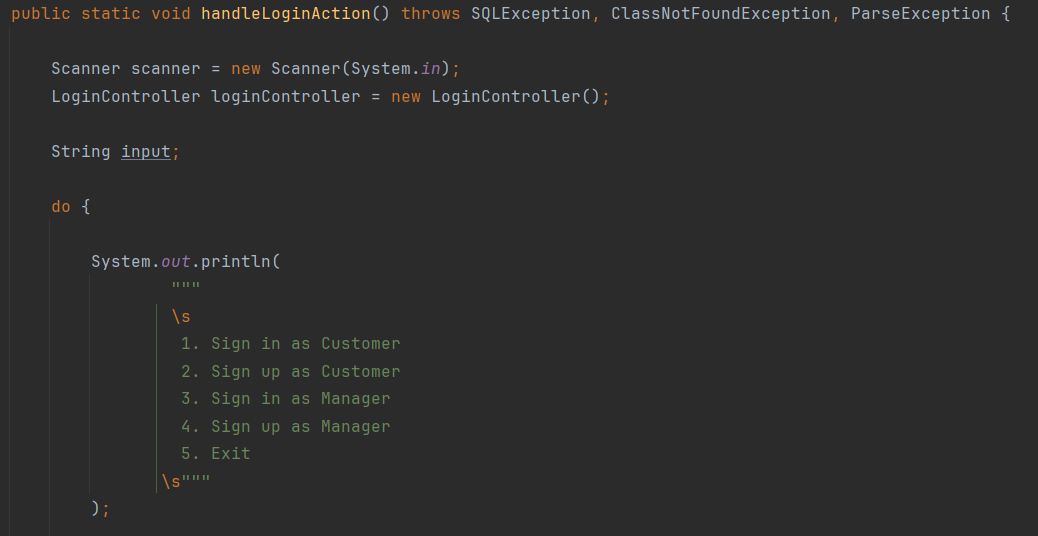
\includegraphics[width=1.0\textwidth]{main.png}
    \caption{Snippet main}
    \label{fig:main}
\end{figure}
\newpage
\section{Testing}
Sono stati realizzati test per verificare il corretto funzionamento del sistema, in particolare
sono stati effettuati dei test funzionali su alcuni metodi del package Business Logic e
dei test strutturali su alcuni metodi del package Domain Model; per il package ORM non
sono stati realizzati test specifici in quanto la correttezza dei metodi `e stata verificata
indirettamente tramite i test sulla logica di business.
\subsection{BusinessLogic Test}
Sono implementati i seguenti test nelle seguenti classi:
\begin{itemize}
    \item LoginControllerTest:\newline
    loginTest(), registerCustomerTest(), registerManagerTest().
    \item CustomerTest:\newline
    BookingOperationsTest(), findRoomTest(), getReviewsTest().
    \item ManagerTest:\newline
    StructureOperationsTest().
\end{itemize}
I test della classe LoginControllerTest verificano il corretto funzionamento dei metodi login(), registerCustomer() e registerManager(), utilizzando utenti noti e nuovi.
\begin{figure}[h!]
    \centering
    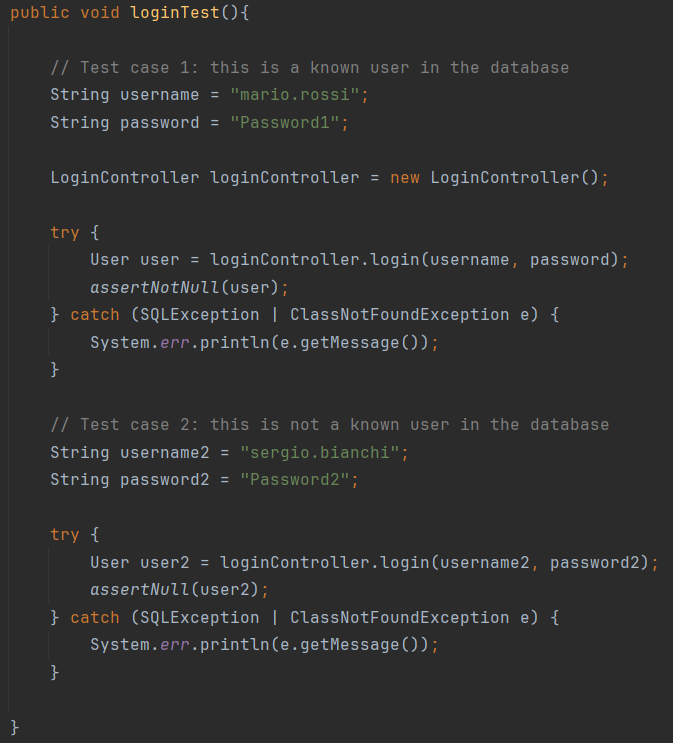
\includegraphics[width=1.0\textwidth]{LoginTest.png}
    \caption{Snippet LoginTest}
    \label{fig:LoginTest}
\end{figure}
\newpage
I test della classe CustomerTest verificano il corretto funzionamento dei metodi bookRoom(), getBooking(), removeSingleBooking(), findRoom(), removesingleRoom(), addReview(), avgHotel(), avgUser removeReview(), utilizzando strutture note e nuove.
\begin{figure}[h!]
    \centering
    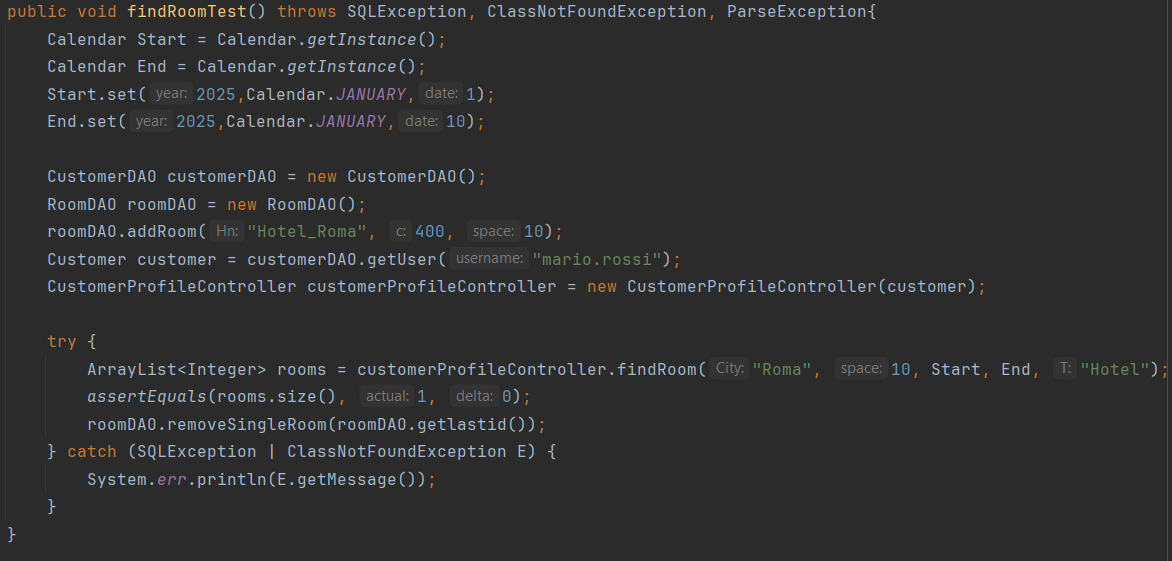
\includegraphics[width=1.0\textwidth]{findRoomTest.png}
    \caption{Snippet findRoomTest}
    \label{fig:findRoomTest}
    \vspace{2mm}
    \centering
    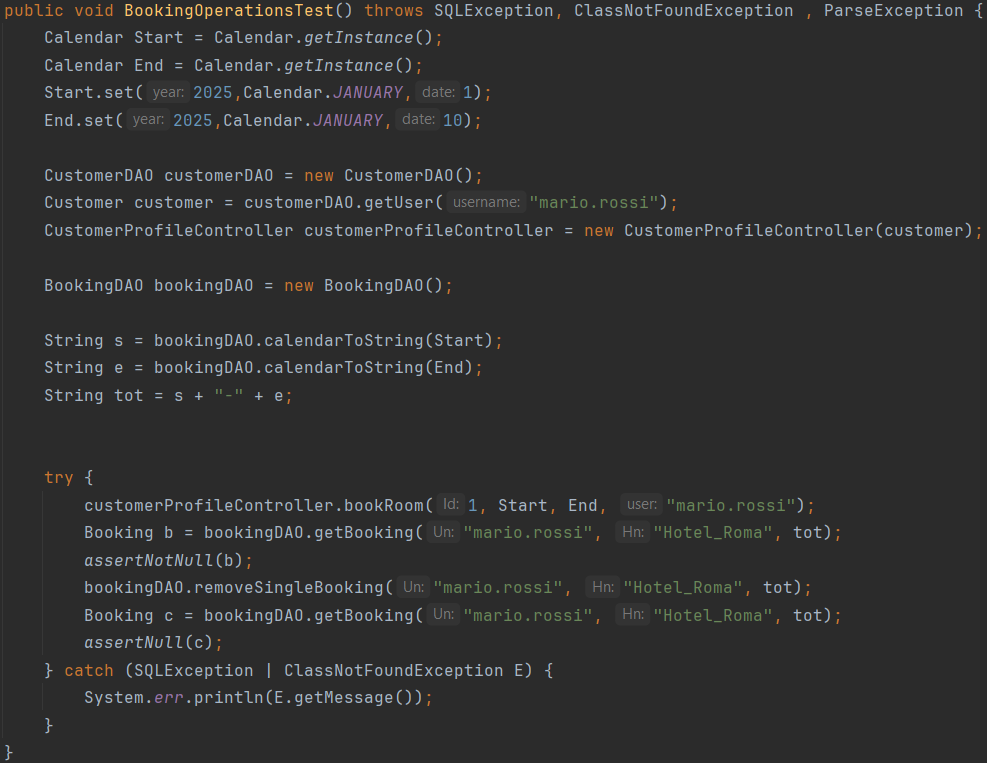
\includegraphics[width=1.0\textwidth]{BookingTest.png}
    \caption{Snippet BookingTest}
    \label{fig:BookingTest}
\end{figure}
\newpage
Il test della classe ManagerTest verifica il corretto funzionamento di addStructure(), getStructure() e removeStructure, tramite una nuova struttura.
\begin{figure}[h!]
    \centering
    \includegraphics[width=1.0\textwidth]{StructureTest.png}
    \caption{Snippet StructureTest}
    \label{fig:StructureTest}
\end{figure}
\newline
\subsection{DomainModel Test}
Sono stati implementati i seguenti test nelle seguenti classi:
\begin{itemize}
    \item CreditCardTest: payTest() e refundTest().
\end{itemize}
Questi test verificano il corretto funzionamento dei metodi di pagamento e rimborso della classe CreditCard. Attraverso la simulazione di un caso noto si
verifica che i passaggi del pagamento e del rimborso avvengano correttamente.
\begin{figure}[h!]
    \centering
    \includegraphics[width=1.0\textwidth]{RefundTest.png}
    \caption{Snippet RefundTest}
    \label{fig:RefundTest}
\end{figure}
\begin{figure}
     \centering
    \includegraphics[width=1.0\textwidth]{PayTest.png}
    \caption{Snippet PayTest}
    \label{fig:PayTest}
\end{figure}
\end{document}
